\documentclass[a4paper,12pt]{article}
\usepackage[utf8]{inputenc}
\usepackage{graphicx}
\usepackage{multicolumn}
\usepackage{multirow}
\usepackage{booktabs}
\usepackage[indent=0pt,skip=3mm]{parskip}
\usepackage{array}
\usepackage{listings}             % Include the listings-package
\usepackage{tabs}
% \usepackage{colortbl}
\usepackage{url}
\usepackage{datetime}
\usepackage[ top=5cm, left=3cm, right=2cm, headheight=4cm]{geometry}
\usepackage{lastpage} % include last page numbering
\usepackage{fancyhdr}
\usepackage[table]{xcolor}% ctan.org/pkg/xcolor %FOR COLORS
% \usepackage{frame}
\settimeformat{ampmtime}
\hyphenation{matriz}
\graphicspath{{figures/}{./images/}}
\newcommand{\eq}[1]{$#1$}
\newcommand{\head}[1]{{\bfseries #1}}
\newcommand{\header}[2][\tiny]{{\bfseries #1 #2}}

%%%%%%%%%%%%%%%%%%%%%%%%%%%%%%%%%%%%%%%%%%%%%%%%%%%%%%%%%%%%%%%%%%%%%%
%%%%%%%%%%%%%%%%%%%%%%%%%%%%%%%%%%%%%%%%%
\newsavebox{\mytabularheader}
\newsavebox{\mytabularheadertitle}
\setlength{\extrarowheight}{0.1cm}
%----------------------------------------------------------------------------------
%-----------------------------------------------------------------------------------------------
\sbox{\mytabularheadertitle}{%
  \begin{minipage}{.52\textwidth}
    \begin{center}
        \bfseries \scriptsize  UNIVERSIDAD NACIONAL DE SAN AGUSTIN\\
        FACULTAD DE INGENIERÍA DE PRODUCCIÓN Y SERVICIOS\\
        ESCUELA PROFESIONAL DE INGENIERÍA DE SISTEMA\\[3mm]
    \end{center}
  \end{minipage}
}

\sbox{\mytabularheader}{%
    \begin{minipage}{\textwidth}
        \centering
        \begin{tabular}{cp{8cm}c}
            
\includegraphics[scale=0.3]{epis_logo.png} & 
            \usebox{\mytabularheadertitle} &
            
\includegraphics[scale=0.05]{abet_logo.png} \\
            % \hline
            \multicolumn{3}{c}{Formato: Guía de Práctica de Laboratorio / Talleres / Centros de Simulación}\\
             &\multicolumn{1}{c}{Aprobación:  2022/03/01 Código: GUIA-PRLE-001} &  \\
        \end{tabular}
    \end{minipage}
}
%---------------------------------------
\renewcommand{\headrulewidth}{0pt}
\fancypagestyle{plain}{%
  \fancyhf{}%
  \fancyhf[ch]{\usebox{\mytabularheader}}
}
%--------------------------------------
\pagestyle{plain}
%%%%%%%%%%%%%%%%%%%%%%%%%%%%%%%%%%%%%%%%%%%%%%%%%%%%%%%%%%%%%%%%%%%%%%%%%%%%%%%%%%%%%%%%%%
\definecolor{blackRed}{cmyk}{0,81,76,31}

\begin{document}    
\lstset{language=Python,frame=single, firstnumber=1,basicstyle=\footnotesize,
numbers=left,showspaces=false,showstringspaces=false}   
    \begin{table}[t]
        \centering
        \begin{tabular}{|p{2.3cm}<{:}|m{1.7cm}|m{2.4cm}|m{2cm}|m{3cm}|m{0.6cm}|}
            \multicolumn{6}{c}{\cellcolor{blackRed}{\leavevmode\color{white}\header{INFORMACIÓN BÁSICA}}}\\
            \hline
            \header{ASIGNATURA} & \multicolumn{5}{c}{\header[\footnotesize]{Física Computacional.}}\\
            \hline
            \header{\mbox{TÍTULO DE LA} PRÁCTICA} & \multicolumn{5}{c}{\header[\footnotesize]{Práctica de Ecuación diferencial de Laplace.}}\\
            \hline
            \header{\mbox{NÚMERO DE} PRÁCTICA} & {\header[\footnotesize]{05}} & \header{AÑO LECTIVO:} & {\header[\footnotesize]{2022-A}} & \header{NRO. SEMESTRE:} & \header[\footnotesize]{VII}\\
            \hline
            \header{\mbox{FECHA DE} \mbox{PRESENTACIÓN}} & \header{\today} & \header{HORA DE \mbox{PRESENTACIÓN:}} & \multicolumn{3}{c}{\header[\footnotesize]{\currenttime}}\\
            \hline
            \multicolumn{4}{l}{\header[\footnotesize]{Integrante(s): Alván Ventura Edsel Yael}} & \header{NOTA} & \\
            \hline
            \multicolumn{6}{l}{\header[\footnotesize]{DOCENTE(s):} \header[\footnotesize]{Danny Giancarlo Apaza Veliz.}} \\  
            \bottomrule
        \end{tabular}
    \end{table}
    \title{Práctica 5\\Física Computacional}
    \date{\vspace{-5ex}}
    \maketitle
    \begin{center}
        Escrito por\\
        Alván Ventura, Edsel Yael\\ \texttt{ealvan@unsa.edu.pe}
        \\[3mm]
        Profesor\\Apaza Veliz, Danny Giancarlo\\ \texttt{dapazav@unsa.edu.pe}\\[3mm]
        \today
    \end{center}
    % \newgeometry{top=2cm}
    \enlargethispage{\baselineskip}
    % \newpage
    \section{Problema 1}
    Resuelva aproximadamente la ecuación de Laplace \eq{\nabla^2u = 0} en un
    cuadrado definido por \eq{0 < x < 4} y \eq{ 0 < y < 4}, con las condiciones en la
    frontera.
    \begin{quote}
        \centering
        \eq{u(x,0) = 20} y \eq{u(x,4) = 300} para todo \eq{0 < x <4}\\
        \eq{u(0,y) = 80} y \eq{u(4,y) = 0} para todo \eq{0 < y <4}
    \end{quote}
    \newpage
    \newgeometry{bottom=1cm,top=5cm,left=2.5cm,right=1.5cm}
    \subsection{Análisis}
    La ecuación diferencial de Laplace puede ser resuelta 
    numéricamente mediante la técnica de 
    diferencias finitas, las diferencias finitas pueden 
    ayudarnos a aproximar mucho a una solución analítica.
    
    Para lograrlo, necesitamos deducir esta formula:
    \begin{equation}
        u(i,j) = \frac{1}{4}(u_{i+1,j}+u_{i-1,j}+u_{i,j-1}+u_{i,j+1})
    \end{equation}
    A partir de las series de taylor, se debe deducir una aproximación numérica a 
    la segunda derivada de la funcion \eq{u(i,j)}:
    \begin{figure}[h]
        \centering
        \includegraphics[width=10cm]{demo1.jpg}
    \end{figure}
    \begin{figure}[h]
        \centering
        \includegraphics[width=10cm]{demo2.jpg}
    \end{figure}
    \newpage
    \subsection{Programación}
    Luego de la deducción:
    \begin{enumerate}
        \item Se creó una matriz de m{\scriptsize x}n.
        \item Los contornos de la matriz se especificaron con las condiciones frontera Dirichtlet dadas por el problema.
        \item Luego, la parte central de la matriz(no incluyendo los bordes) 
        se lleno de la media de los valores de las condiciones frontera Dirichtlet(\eq{(xu+xd+yl+yd)/4}).
        \item Despues de hacer eso, se implementó la técnica numérica para iterar sobre la parte central de la matriz anteriormente dicha.
        \item Y finalmente, se colocó la matriz en un mapa de calor, para ver las condiciones frontera(se uso la librería \emph{matplotlib}).
    \end{enumerate}

    Cabe destacar que las dimensiones del array son parámetros 
    de la función llamada \eq{Laplace()}.

    Esta función se denota de la siguiente manera:
    \begin{equation}
        %err aun no me sale, esta F, no converge en esa variable
        Laplace(xu,xd,yl,yr,f,c,h)
    \end{equation}
    Donde:
        \begin{table}[h]
            \centering
            \begin{tabular}{>{\footnotesize}l<{:}>{\footnotesize}p{6cm}>{\footnotesize}p{4cm}<{ del cuadrado}}
            \toprule
            \head{Parámetros} & \multicolumn{2}{c}{\head{Descrición}}\\
            \midrule
            xu & Representa la recta \eq{u(x,4) = 300 = xu}& Arriba\\
            xd & Representa la recta \eq{u(x,0) = 20 = xd}& Abajo\\
            yl & Representa la recta \eq{u(0,y) = 80 = yl}& Izquierda\\
            yr & Representa la recta \eq{u(4,y) = 300 = yr}& Derecha\\
            f & Representa el número de filas de la matriz\\
            c & Representa el número de columnas de la matriz\\
            h & Representa el número de iteraciones de la matriz\\
            % err&Representa el error minimo que se debe obtener.\\
            % \bottomrule
            \end{tabular}
        \end{table}

    A continuación se muestra la implementación:
    
    \lstinputlisting[label=Archivo ejer1.py]{ejer1.py}
    
    Como se puede ver, los datos del primer ejercicio estan puestos en la siguiente pieza de código:
    \lstinputlisting[label=Archivo ejer1.py,firstline=43, lastline=51]{ejer1.py}

    \subsection{Resultados}
        Los resultados son los siguientes:
        \begin{figure}[h]
            \centering
            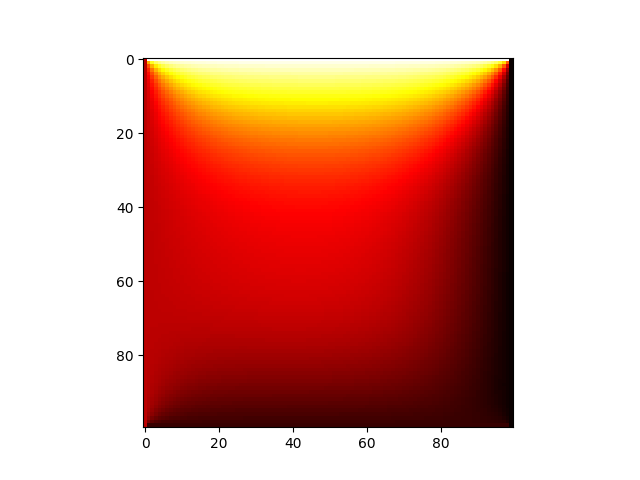
\includegraphics[scale=0.7]{ejer1_demostr.png}
            \caption{Mapa de calor del problema 1.}
        \end{figure}

        En la anterior imagen se puede ver, los puntos mas calientes, donde 
        la función alcanza sus valores máximos(color rojizo anaranjado),
        y la parte negra representa los valores mínimos de la función.
    \section{Problema 2}
    Use y modifique el código del ejercicio 1 y calcule las aproximaciones
    de la función \eq{u(x, y)} en el cuadrado cuadrado definido por \eq{0 < x < 4} y
    \eq{0 < y < 4}, con las condiciones en la frontera.
    \begin{quote}
        \centering
        \eq{u(x,0) = 120} y \eq{u(x,4) = 0} para todo \eq{0 < x < 4}\\
        \eq{u(0,y) = 120} y \eq{u(4,y) = 0} para todo \eq{0 < y < 4}
    \end{quote}
    \subsection{Análisis}
    En la siguiente tabla se especifica, qué valores se tomaron para el problema 2,
    a partir de la implementación del problema 1:
    \begin{table}[t]
        \centering
        \begin{tabular}{>{\footnotesize}l<{:}>{\footnotesize}p{6cm}>{\footnotesize}p{4cm}<{ del cuadrado}}
        \toprule
        \head{Parámetros} & \multicolumn{2}{c}{\head{Descripción}}\\
        \midrule
        xu & Será \eq{u(x,4) = 0 = xu}&arriba\\
        xd & Será la recta \eq{u(x,0) = 120 = xd}&abajo\\
        yl & Será la recta \eq{u(0,y) = 120 = yl}&izquierda\\
        yr & Será la recta \eq{u(4,y) =  0 = yr}&derecha\\
        f & 100 filas para la matriz\\
        c & 100 columnas para la matriz\\
        h & 1000 iteraciones de la matriz\\
        % err&Representa el error minimo que se debe obtener.\\
        % \bottomrule
        \end{tabular}
    \end{table}
    \newpage
    \subsection{Programación}
    La implementación es la misma que el anterior problema, la diferencia radica en los siguientes
    valores dados en esta tabla:
    % \newpage
    \lstinputlisting[firstline=43, lastline=52]{ejer2.py}

    \subsection{Resultados}
    El resultado es el siguiente:
    \begin{figure}[h]
        \centering
        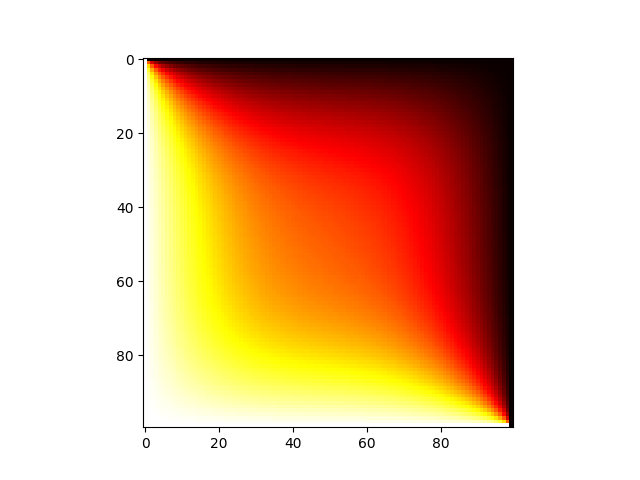
\includegraphics[width=9cm]{ejer2_demostr.PNG}
        \caption{Mapa de calor del problema 2.}
    \end{figure}

    % Como se puede apreciar en la anterior figura, %NO LO HE PROBADO AÚN

    \section{Problema 3}
    Implementar un código computacional para la solución del siguiente
    potencial:
    \begin{equation}
        V(x,y) = \frac{4}{\pi} \sum_{n=1,3,5\dots} ^{\infty} \frac{1}{n} (\frac{V_2 sinh(\frac{n\pi}{b} x) + V_1 sinh(\frac{n\pi}{b}(a-x))}{sinh(\frac{n\pi}{b}a)})sin(\frac{n\pi}{b}y)
    \end{equation}    
    \subsection{Análisis}
    La anterior función es la solucion de una ecuación diferencial, debido a esto, debemos implementar
    gráficamente la función pero análiticamente(debido a que la función es análitica).

    Para lograr esto, debemos tener en cuenta los parámetros de la función:
    
    \begin{table}[h]
        \centering
        \begin{tabular}{ll<{.}}
            \head{Variables y constantes} & \head{Descrición}\\
            \midrule
            \eq{V_1} & Potencial 1\\
            \eq{V_2} & Potencial 2\\
            a & Distancia entre las dos laminas\\
            b & Anchura de las dos láminas\\
            \eq{sinh()} & Se refiere a la funcion hiperbólica de la función seno(\eq{sin()})\\
            x,y & son los parámetros de la función en el plano cartesiano
        \end{tabular}
    \end{table}

    \subsection{Programación}
    Para la implementación del algoritmo se procedió de la siguiente manera:
    
    \begin{enumerate}
        \item Se creó la matriz de m{\scriptsize x}n (por defecto todos los valores en 0).
        \item Después, se recorrió la matriz en toda su extensión con dos \emph{for} anidados(uno para fila y el otro para las columnas).
        \begin{itemize}
            \item Mientras se hacia el paso anterior(dentro de 
            los dos \emph{for}), se usó la función implementada a partir 
            de la solución analítica de la función(\eq{V(x,y)}) 
            con los valores \eq{(x,y)} del plano cartesiano.
        \end{itemize}
        \item Todos estos valores se guardaban respectivamente en la matriz.
        \item Luego se puso la matriz en un mapa de calor(se uso la librería \emph{matplotlib}).
    \end{enumerate}

    A continuación, se muestra la implementación:
    
    \lstinputlisting[label=Archivo ejer3.py]{ejer3.py}

    \subsection{Resultados}
    Los resultados para la función analítica son:
    \begin{figure}[h]
        \centering
        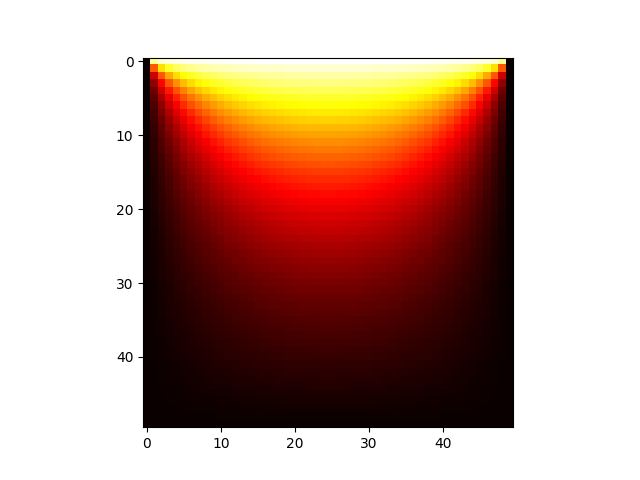
\includegraphics[scale=0.8]{eje3_demostr1.PNG}
        \caption{Mapa de calor del problema 3.}
    \end{figure}
    \section{Anexos}
    Aqui se muestran algunas imágenes en ejecución:
    \subsection{Ejercicio 1:}
    \begin{figure}[h]
        \centering 
        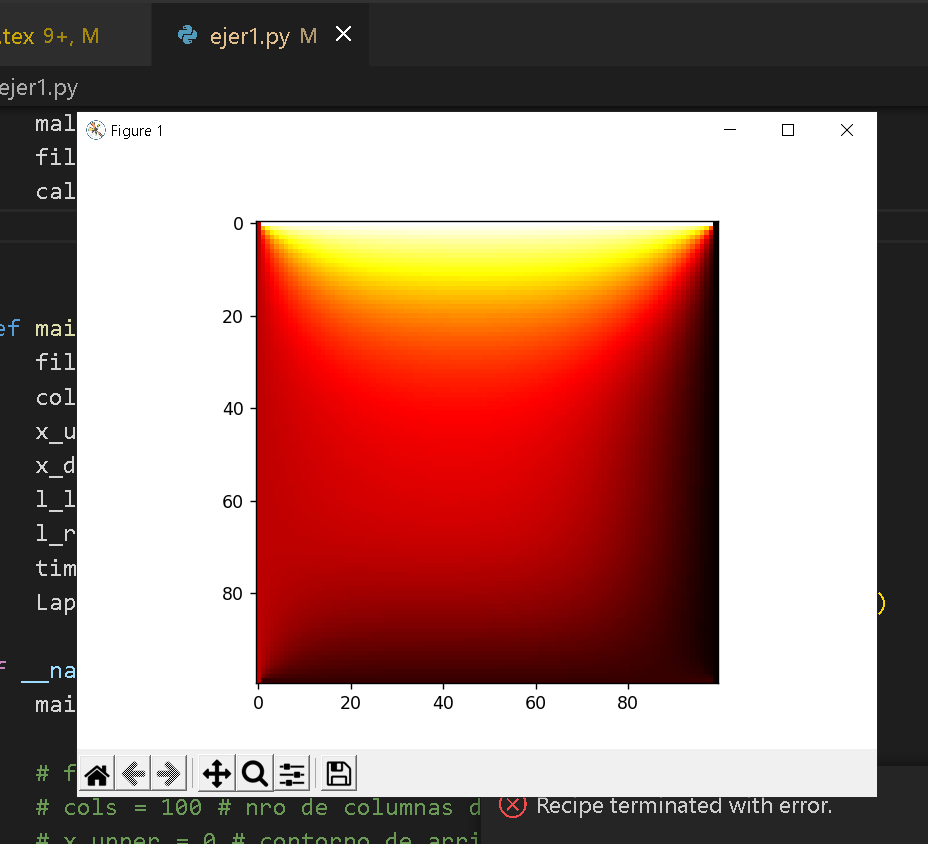
\includegraphics[width=6cm]{ejer1_demostr2.png}
    \end{figure}
	\newpage
    \subsection{Ejercicio 2:}
    \begin{figure}[h]
        \centering 
        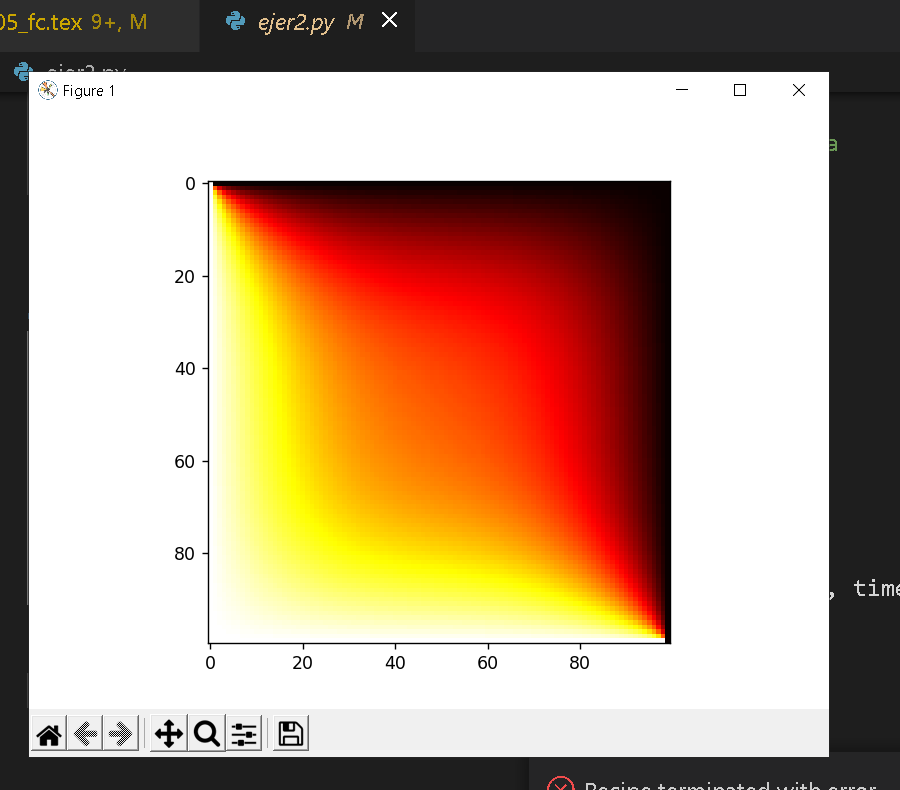
\includegraphics[width=6cm]{ejer2_demostr1.png}
    \end{figure}

    \subsection{Ejericio 3:}
    \begin{figure}[h]
        \centering 
        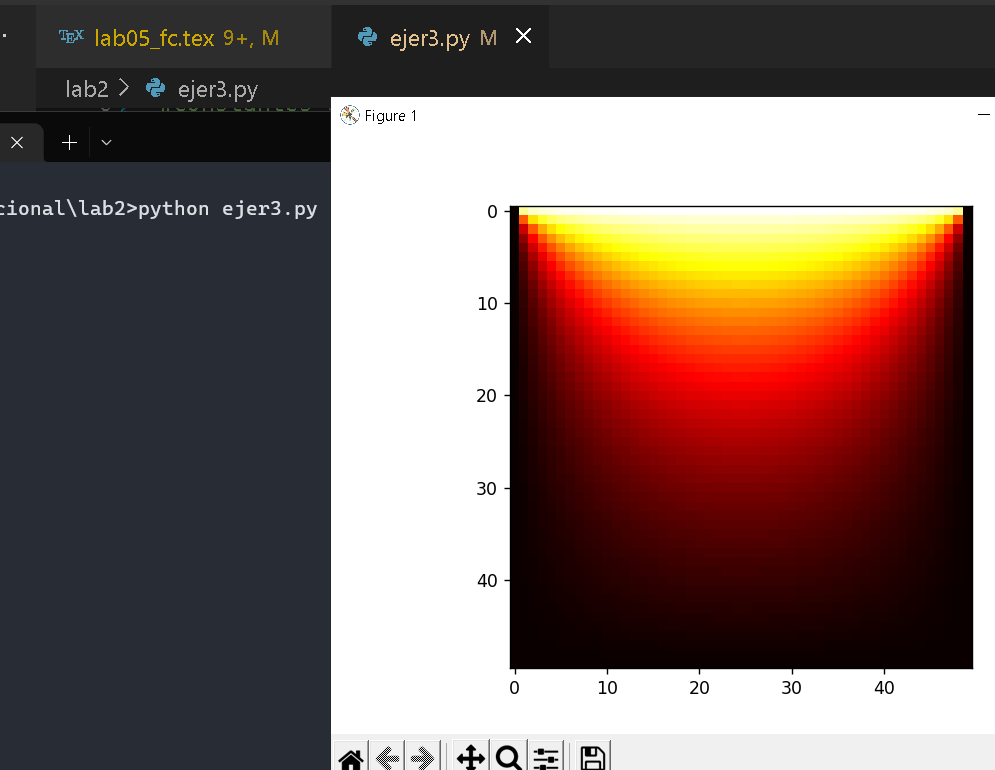
\includegraphics[width=6cm]{eje3_demostr.PNG}
    \end{figure}
    
    


\end{document}
